\documentclass[8pt]{beamer}

\setbeamertemplate{background canvas}[vertical shading][bottom=cyan!10,top=blue!10]

\usetheme{Warsaw}
\usefonttheme[onlysmall]{structurebold}

% pour le fichiers .pdf
\usepackage{graphicx}
\usepackage{color}
% pour les fichiers .png
% \usepackage{pgf,pgfarrows}
% \usepackage{pgf,pgfarrows}
\usepackage{amsmath,amssymb}
\usepackage[latin1]{inputenc}
\usepackage[T1]{fontenc}
\usepackage[french]{babel}
\usepackage{textcomp}
\usepackage{multitoc}
\usepackage{mdwtab}
\setbeamercovered{dynamic}
\DeclareMathOperator*{\argmin}{argmin}

\title[OpenTURNS modules development]{OpenTURNS modules development}
\author[R. Lebrun, copyright EADS 2011.]
{
  Trainer : R�gis LEBRUN\\
  EADS/IW/SE/AM \\
  regis.lebrun@eads.net
}



\date[March 22-25th 2011]
{
  Developers training \\

  \begin{center}
    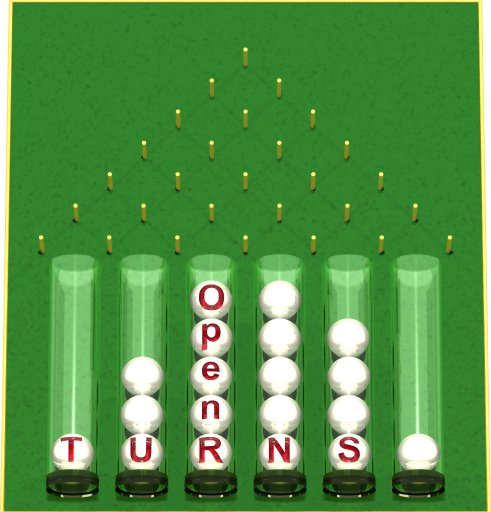
\includegraphics[height=2cm]{logoOT.jpg}
  \end{center}
}

\subject{OpenTURNS Developers Training}

% \part<presentation>{Corps de presentation}


\begin{document}

\frame{\titlepage}

% necessaire pour la table des matieres
\part{Main part}

% table des matieres
\begin{frame}
  \frametitle{OpenTURNS modules development}
  \tableofcontents[part=1]
\end{frame}
%%%%%%%%%%%%%%%%%%%%%%%%% 
% The OpenTURNS package %
%%%%%%%%%%%%%%%%%%%%%%%%% 
\section[OpenTURNS modules]{OpenTURNS modules}
%%%%%%%%%%%%% 
% The tools %
%%%%%%%%%%%%% 
\begin{frame}
  \frametitle{OpenTURNS modules}
  \begin{block}{Objectives}
    OpenTURNS is a growing system developed by a small team. A constant problem is to assess the stability of the whole product, and in order to achieve this goal we introduced a notion of module, in order to insulate a core library dedicated to the definition of the abstract data model and to propose all the specific algorithms as optional modules. The core would evolve quite slowly, insuring its robustness, whereas the modules would have a more dynamic development model.\\
    Another key objective is to provide a way to extend the existing platform with functionalities developed by teams that are reluctant to adopt the OpenTURNS development process. Within the module, the development team can adopt any coding rule or programming language he want, as long as the OpenTURNS interface is respected as well as the objects lifecycle.
  \end{block}
\end{frame}
\begin{frame}
  \frametitle{OpenTURNS modules}
  \centering \resizebox{!}{4cm}{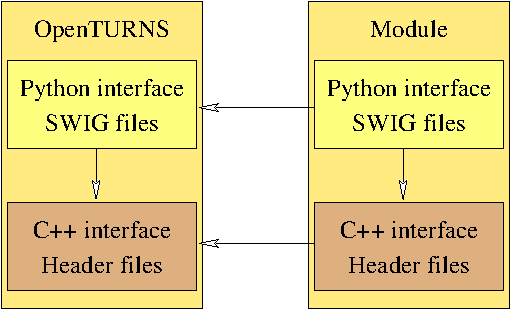
\includegraphics{OTModule.pdf}}
  \begin{block}{The principles}
    An OpenTURNS module is typically made of two parts:
    \begin{itemize}
    \item a C++ part that uses the OpenTURNS C++ interface in order to provide new specialization or to produce instances of the data model using new algorithms with no OpenTURNS counterpart.
    \item a Python part, the Python interface of the C++ part, often obtained using SWIG. In this case, this SWIG interface must use the OpenTURNS interface the same way its C++ interface uses the OpenTURNS C++ interface.
    \end{itemize}
  \end{block}
\end{frame}
\begin{frame}
  \frametitle{OpenTURNS modules}
  \begin{block}{And fo a Python module?}
    For now, there is (almost) no way to use a Python object within the OpenTURNS C++ library. The concept of "OpenTURNS Python module" is not very specific: any set of Python classes or Python functions that use the OpenTURNS Python interface can be called an OpenTURNS Python module. In this case, the notion of OpenTURNS module is mainly a packaging notion, and the use of the Python setup tools is probably more mature and more adapted!
  \end{block}
\end{frame}
\section[Module development]{Module development}
\begin{frame}
  \frametitle{Module development}
  \begin{block}{Step 1: copy and adapt an existing template}
    \begin{itemize}
    \item Copy and rename the source tree of an example module (for example the Strange module) from the OpenTURNS source tree. The examples modules are located under the module subdirectory of OpenTURNS source tree:\\

      {\ttfamily svn export https://svn.openturns.org/openturns-modules/template MyModule}
    \item Adapt the template to your module:\\
      {\ttfamily ./customize MyModule}\\
      This command change the module name into all the scripts, and adapt the example class to this new name.
    \end{itemize}
  \end{block}
\end{frame}

\begin{frame}
  \frametitle{Module development}
  \begin{block}{Step 2: develop the module}
    \begin{itemize}
    \item Implement your module. You are free to use the rules you want, but if the final objective of the module is to be integrated in the official release of OpenTURNS, it is wise to adopt the OpenTURNS development process and rules.
    \item Build your module as usual:
      \begin{tabular}{l}
        \ttfamily ./bootstrap\\
        \ttfamily mkdir build\\
        \ttfamily cd build\\
        \ttfamily ../configure --with-swig=SWIG\_INSTALLDIR \\
        \ttfamily --with-openturns=OPENTURNS\_INSTALLDIR\\
        \ttfamily make
      \end{tabular}
    \item Create a source package of your module:\\
      {\ttfamily make dist}\\
      It will create a tarball named mymodule-X.Y.Z.tar.gz (and mymodule-X.Y.Z.tar.bz2), where X.Y.Z is the version number of the module.
    \end{itemize}
  \end{block}
\end{frame}

\begin{frame}
  \frametitle{Module development}
  \begin{block}{Step 3: install and test the module}
    \begin{itemize}
    \item Check that you have a working OpenTURNS installation, for example by trying to load the OpenTURNS module within an interactive python session:
      \begin{tabular}{l}
        \ttfamily python\\
        \ttfamily >>> from openturns import *\\
      \end{tabular}

      and python should not complain about a non existing openturns module.
    \item In the python directory of the OpenTURNS install directory, you can find a script named {\itshape openturns-module}. You use this script to install the tarball mymodule.tar.gz (or mymodule.tar.bz2) in your home directory ({\itshape \$HOME/openturns}):\\
      {\ttfamily openturns-module --install=mymodule-X.Y.Z.tar.gz --prefix=user}\\
      The installation script has many more capabilities, you can access to its embedded documentation by invoking it without argument.
    \item Test your module within python:\\
      \begin{tabular}{l}
        \ttfamily python \\
        \ttfamily >>> from openturns import * \\
        \ttfamily >>> from mymodule import * \\
      \end{tabular}

      and python should not complain about a non existing mymodule module.
    \end{itemize}
  \end{block}
\end{frame}

\begin{frame}
  \frametitle{Module development}
  \begin{block}{OpenTURNS module management}
    \scriptsize
    \begin{tabular}{l}
      \ttfamily openturns-module \\
      \ttfamily Usage: openturns-module [--silent] {--install=<module> | --remove=<module>} [--prefix=PFX] [extra\_configure\_args] \\
      \ttfamily openturns-module [--silent] {--install <module> | --remove <module>} [--prefix PFX] [extra\_configure\_args] \\
      \ttfamily  openturns-module [--silent] {--module=<module> | --module <module>} [options] \\
      \ttfamily  Note: \\
      \ttfamily For installation, 'module' can be either a path to a directory \\
      \ttfamily  or a path to a archive file (compressed or not). \\
      \ttfamily For removal, 'module' is the module name. \\
      \ttfamily The extra configure args are passed as is to the module configure \\
      \ttfamily script. \\
      \\
      \ttfamily Example: \\
      \ttfamily (install) \\
      \ttfamily openturns-module --install=mymodule/ \\
      \ttfamily openturns-module --install=/path/to/mymodule/ \\
      \ttfamily openturns-module --install=mymodule.tar \\
      \ttfamily openturns-module --install=mymodule.tar.gz \\
      \ttfamily openturns-module --install=mymodule.tgz \\
      \ttfamily openturns-module --install=mymodule.tar.bz2 \\
      \ttfamily openturns-module --install=mymodule.tbz \\
      \\
      \ttfamily You can provide a prefix to choose where the module will be installed. \\
      \ttfamily PFX can take one of the following values: \\
      \ttfamily * openturns : the module will be installed in the Open TURNS installation tree
    \end{tabular}
  \end{block}
\end{frame}
\begin{frame}
  \frametitle{Module development}
  \begin{block}{OpenTURNS module management}
    \scriptsize
    \begin{tabular}{l}
      \ttfamily * user : the module will be installed in the Open TURNS user directory (/home/regis/openturns) \\
      \ttfamily * <dir> : the module will be installed in <dir>. You should append <dir> to the \\
      \ttfamily OPENTURNS\_MODULE\_PATH envvar to tell Open TURNS where to find the module \\
      \\
      \ttfamily (remove) \\
      \ttfamily openturns-module --remove=mymodule \\
      \\
      \ttfamily (mixed form) \\
      \ttfamily openturns-module --remove=myoldmodule1 --install=mynewmodule1 --install=mymodule2 \\
      \ttfamily (module) \\
      \ttfamily openturns-module --module=mymodule \\
      \\
      \ttfamily Options: \\
      \ttfamily --silent          Do not output any message \\
    \end{tabular}
  \end{block}
\end{frame}
\end{document}